\documentclass{article}

\usepackage{algorithmic, amsmath, amsthm, amsfonts, amssymb,commath,  enumerate, tikz, tikz-cd, color, mathrsfs} %tikz is for drawing lattices %tikz-cd is for commutative diagrams
															%color is for making notes in red 
															%mathrsfs is for power set font
%\usepackage[mathscr]{eucal} %mathscr gives nice script fonts

\newtheoremstyle{problemstyle}  % <name> This is my problemstyle. use begin{problem}.
        {12pt}                                               % <space above>
        {}                                               % <space below>
        {\itshape}                               % <body font>
        {}                                                  % <indent amount}
        {\bfseries}                 % <theorem head font>
        {\normalfont\bfseries.}         % <punctuation after theorem head>
        {.5em}                                          % <space after theorem head>
        {}                                                  % <theorem head spec (can be left empty, meaning `normal')>


\theoremstyle{problemstyle}

\newtheorem{problem}{Problem}

\definecolor{purple}{rgb}{1,0,1}

\title{ \vspace{-10ex} %uncomment to remove vertical space
%title of assignment goes here e.g. "Math 721 Homework 3"
Math 260 Lecture 1 Introduction
}


\author{David L. Meretzky
}


\date{%date assignment is due goes here
Monday August 27th, 2018
} 


\renewcommand*{\thefootnote}{$\dagger$} %changes default footnote marking to a dagger instead of a number (numbers are sometimes mistaken for citations)

\begin{document}

\maketitle

\section{$\mathbb{R}^n$ and $\mathbb{C}^n$}

\subsection{Introduction}

Vectors as known from Calculus or Physics are geometric objects. They represent quantities with magnitude and direction, and consequently a natural way to draw them is as arrows. 
Frequently, one has to add vectors. This vector addition behaves somewhat like the addition of real numbers, that is, given two numbers, adding them gives us back a real number. Vector addition should work the same way.  Given two vectors $u$ and $v$, the way we add them is by composing them to get a third vector as shown below:  $$\textcolor{red}{u} + \textcolor{blue}{v} = \textcolor{purple}{w}$$ 

%% FIG 1 %%
\begin{center}
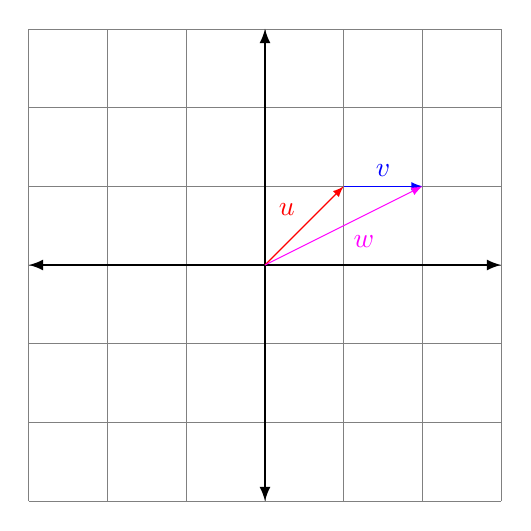
\begin{tikzpicture}[commutative diagrams/every diagram]
\draw [help lines] (-3,-3) grid (3,3);

% axes
\draw[-latex, thick] (0,0) to (3,0); 
\draw[-latex, thick] (0,0) to (0,3);
\draw[-latex, thick] (0,0) to (-3,0); 
\draw[-latex, thick] (0,0) to (0,-3); 

\draw[-latex, thin,red] (0,0) to["$u$", red] (1,1) ;
\draw[-latex, thin,blue] (1,1) to["$v$", blue] (2,1) ;
\draw[-latex, thin,purple] (0,0) to[swap, "$w$", purple] (2,1) ;
\end{tikzpicture}
\end{center}
%% END FIG 1 %%

The notation $u+v$ is certainly curious in this context. Might it be clearer to use the usual notation for function composition $v\circ u$ meaning "apply $v$ to $u$" or "follow $u$ with $v$"? Also, does the order matter? In our experience with functions often $f \circ g \neq g \circ f$. Let $f(x) = x + 3$ and let $g(x) = x^2$. Then $f\circ g (x) = f(g(x)) = f(x^2) = x^2 + 3$ while $g \circ f (x) = g(f(x)) = g(x+3) = (x+3)^2 = x^2 + 6x + 9$. 

If we use the geometry of our picture then we can certainly verify for these example vectors that $$\textcolor{red}{u} + \textcolor{blue}{v} = \textcolor{blue}{v}+\textcolor{red}{u}$$

%% FIG 2 %%
\begin{center}
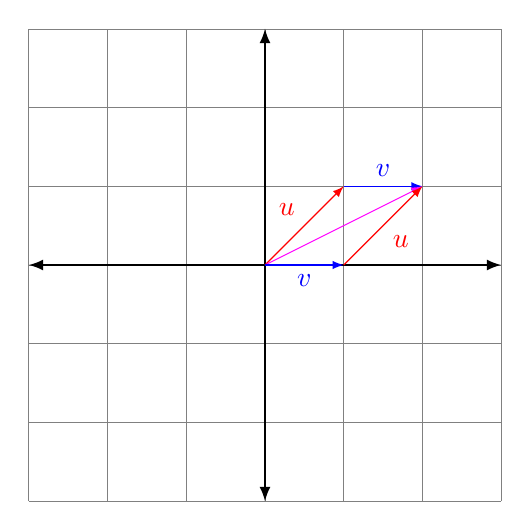
\begin{tikzpicture}[commutative diagrams/every diagram]
\draw [help lines] (-3,-3) grid (3,3);

% axes
\draw[-latex, thick] (0,0) to (3,0); 
\draw[-latex, thick] (0,0) to (0,3);
\draw[-latex, thick] (0,0) to (-3,0); 
\draw[-latex, thick] (0,0) to (0,-3); 

\draw[-latex, thin,red] (0,0) to["$u$", red] (1,1) ;
\draw[-latex, thin,blue] (1,1) to["$v$", blue] (2,1) ;
\draw[-latex, thin,purple] (0,0) to [purple] (2,1) ;
\draw[-latex, thin,blue] (0,0) to["$v$",swap, blue] (1,0) ;
\draw[-latex, thin,red] (1,0) to["$u$",swap, red] (2,1) ;
\end{tikzpicture}
\end{center}
%% END FIG 2 %%

What is it about the geometry of the plane that makes this vector addition commutative? It turns out that this commutativity is exactly our intuitive notion of straightness.  It is the $absence$ $of$ $curvature$ which makes vector addition commutative.\\

Suppose instead of the plane, our vectors live on the surface of a sphere. If we let the vector $v$ correspond to moving $1$ unit length horizontally (parallel to the lines of latitude), and $u$ correspond to moving $1$ unit length vertically (parallel to the lines of longitude), then it is simple to check that $u+v \neq v+u$. Notice that on the equator the lines of longitude are exactly $1$ unit apart, but above or below it they are less than $1$ unit apart.\\ 

$\textit{Draw in sphere examples from class:}$\\\\\\\\\\\\

A collection of vectors which satisfies certain algebraic properties (one of which is the commutativity of vector addition) is called a $vector$ $space$.  Vector spaces and the structure-preserving functions between them (the functions which take vector spaces to vector spaces) are the principal objects of study in Linear Algebra. Although most of our examples will come from $\mathbb{R}^n$ or similar vector spaces with visual interpretations, vector spaces are abstract structures which do not actually have to be composed of vectors with a physical or visual interpretation. Each of the algebraic properties of a vector space corresponds to a physical interpretation.  For example, the commutativity of vector addition corresponds to a lack of curvature of the space. Although the abstract point of view will be emphasized, vector spaces lend themselves very nicely to computation even in very abstract cases.
\end{document}
